\documentclass[spanish]{beamer}
\usepackage[ansinew]{inputenc} % Acepta caracteres en castellano
\usepackage[spanish]{babel}    % silabea palabras castellanas
\usepackage{amsmath}
\usepackage{mathtools,cancel} % cancela con una flecha \cancelto{0}{XXXX}
\renewcommand{\CancelColor}{\color{red}} %change cancel color to red
\usepackage{amsfonts}
\usepackage{amssymb}
\usepackage{dsfont}
\usepackage{graphicx}
\usepackage{geometry}
\usetheme{Madrid}
\usecolortheme{beaver}
\usepackage{textpos}
% Logo  en el comienzo 
\addtobeamertemplate{frametitle}{}{%
\begin{textblock*}{100mm}(.85\textwidth,-1cm)
{\includegraphics[height=0.4in, keepaspectratio=true]{/Users/luisnunez/Dropbox/MisDocumentos/UIS/UISImagenInstitucional/UISLOGO.png}}
\end{textblock*}}

\begin{document}

\title{\textbf{Hamilton Jacobi} }
\author[L.A. N��ez]{\textbf{Luis A. N��ez}}  
\institute[UIS]{\textit{Escuela de F�sica, Facultad de Ciencias, } \\
\textit{Universidad Industrial de Santander, Santander, Colombia } \\
{\includegraphics[height=0.4in, keepaspectratio=true]{/Users/luisnunez/Dropbox/MisDocumentos/UIS/UISImagenInstitucional/UISLOGO.png}}
}
\date{\today}
\maketitle


\begin{frame}
\frametitle{Agenda}
  \tableofcontents
\end{frame}


%%%%% Diapo 1
\section{Ecuaci�n de Hamilton Jacobi}
\frame{
  \frametitle{Ecuaci�n de Hamilton Jacobi}
   \begin{itemize}  
  	\item<1-> Una transformaci�n can�nica $Q_i=Q_i\left(q_j, p_j, t\right), P_i=P_i\left(q_j, p_j, t\right)$, permite encontrar las soluciones de las ecuaciones de Hamilton.
	\item<2-> Esa transformaci�n $Q_i=Q_i\left(q_j, p_j, t\right), P_i=P_i\left(q_j, p_j, t\right)$ lleva $\mathcal{H}\left(q_j, p_j, t\right)\leftarrow \mathcal{H}^{\prime}\left(Q_i, P_i, t\right)$ con $\mathcal{H}^{\prime}\left(Q_i, P_i, t\right)$ un hamiltoniano en el cual alguna (o varias) coordenada $Q_j$ o $P_j$ son c�clicas
	\item<3-> Tenemos una transformaci�n can�nica $\left\{q_i, p_i, t\right\} \rightarrow \left\{P_i, Q_i, t\right\}$ tal que las $2 s$ nuevas coordenadas y momentos $\left(P_i, Q_i\right)$ son constantes.
	\item<4-> Esas $2 s$ cantidades constantes $Q_i$ y $P_i$ pueden expresarse en funci�n de las $2 s$ condiciones iniciales $\left(q_i(0), p_i(0)\right)$; es decir, $Q_i=q\left(q_j(0), p_j(0)\right), P_i=p\left(q_j(0), p_j(0)\right)$.
    \end{itemize}
}

%%%%% Diapo 2
\section{Secci�n}
\frame{
\frametitle{T�tulo transparencia}
\begin{itemize}  
	\item<1-> 
\end{itemize}
}

%%%%% Diapo Fin
\section{Recapitulando}
\frame{
  \frametitle{Recapitulando}
En presentaci�n consideramos
  \begin{enumerate}
  	\item<1->
   \end{enumerate}
}
  
\end{document}

	\begin{figure}[t]
		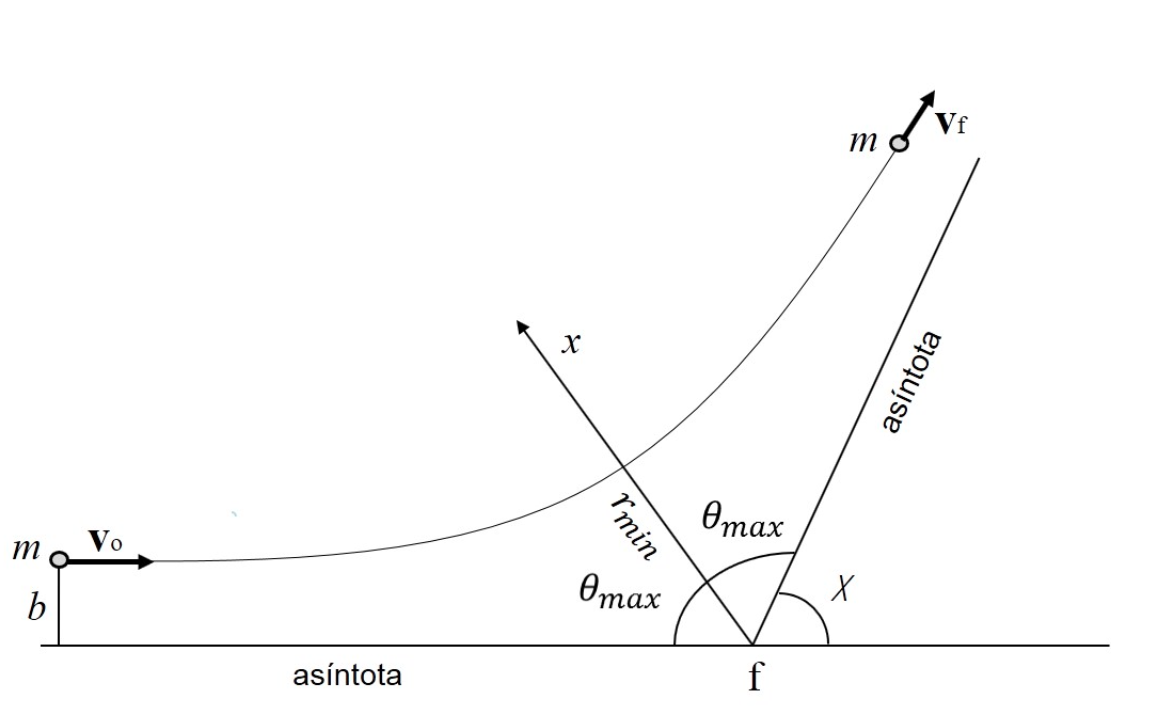
\includegraphics[width=1.8in]{Figuras/Dispersion.png}
   	\end{figure}
	
